% Options for packages loaded elsewhere
\PassOptionsToPackage{unicode}{hyperref}
\PassOptionsToPackage{hyphens}{url}
\PassOptionsToPackage{dvipsnames,svgnames,x11names}{xcolor}
%
\documentclass[
  letterpaper,
  DIV=11,
  numbers=noendperiod]{scrartcl}

\usepackage{amsmath,amssymb}
\usepackage{iftex}
\ifPDFTeX
  \usepackage[T1]{fontenc}
  \usepackage[utf8]{inputenc}
  \usepackage{textcomp} % provide euro and other symbols
\else % if luatex or xetex
  \usepackage{unicode-math}
  \defaultfontfeatures{Scale=MatchLowercase}
  \defaultfontfeatures[\rmfamily]{Ligatures=TeX,Scale=1}
\fi
\usepackage{lmodern}
\ifPDFTeX\else  
    % xetex/luatex font selection
\fi
% Use upquote if available, for straight quotes in verbatim environments
\IfFileExists{upquote.sty}{\usepackage{upquote}}{}
\IfFileExists{microtype.sty}{% use microtype if available
  \usepackage[]{microtype}
  \UseMicrotypeSet[protrusion]{basicmath} % disable protrusion for tt fonts
}{}
\makeatletter
\@ifundefined{KOMAClassName}{% if non-KOMA class
  \IfFileExists{parskip.sty}{%
    \usepackage{parskip}
  }{% else
    \setlength{\parindent}{0pt}
    \setlength{\parskip}{6pt plus 2pt minus 1pt}}
}{% if KOMA class
  \KOMAoptions{parskip=half}}
\makeatother
\usepackage{xcolor}
\setlength{\emergencystretch}{3em} % prevent overfull lines
\setcounter{secnumdepth}{-\maxdimen} % remove section numbering
% Make \paragraph and \subparagraph free-standing
\makeatletter
\ifx\paragraph\undefined\else
  \let\oldparagraph\paragraph
  \renewcommand{\paragraph}{
    \@ifstar
      \xxxParagraphStar
      \xxxParagraphNoStar
  }
  \newcommand{\xxxParagraphStar}[1]{\oldparagraph*{#1}\mbox{}}
  \newcommand{\xxxParagraphNoStar}[1]{\oldparagraph{#1}\mbox{}}
\fi
\ifx\subparagraph\undefined\else
  \let\oldsubparagraph\subparagraph
  \renewcommand{\subparagraph}{
    \@ifstar
      \xxxSubParagraphStar
      \xxxSubParagraphNoStar
  }
  \newcommand{\xxxSubParagraphStar}[1]{\oldsubparagraph*{#1}\mbox{}}
  \newcommand{\xxxSubParagraphNoStar}[1]{\oldsubparagraph{#1}\mbox{}}
\fi
\makeatother

\usepackage{color}
\usepackage{fancyvrb}
\newcommand{\VerbBar}{|}
\newcommand{\VERB}{\Verb[commandchars=\\\{\}]}
\DefineVerbatimEnvironment{Highlighting}{Verbatim}{commandchars=\\\{\}}
% Add ',fontsize=\small' for more characters per line
\usepackage{framed}
\definecolor{shadecolor}{RGB}{241,243,245}
\newenvironment{Shaded}{\begin{snugshade}}{\end{snugshade}}
\newcommand{\AlertTok}[1]{\textcolor[rgb]{0.68,0.00,0.00}{#1}}
\newcommand{\AnnotationTok}[1]{\textcolor[rgb]{0.37,0.37,0.37}{#1}}
\newcommand{\AttributeTok}[1]{\textcolor[rgb]{0.40,0.45,0.13}{#1}}
\newcommand{\BaseNTok}[1]{\textcolor[rgb]{0.68,0.00,0.00}{#1}}
\newcommand{\BuiltInTok}[1]{\textcolor[rgb]{0.00,0.23,0.31}{#1}}
\newcommand{\CharTok}[1]{\textcolor[rgb]{0.13,0.47,0.30}{#1}}
\newcommand{\CommentTok}[1]{\textcolor[rgb]{0.37,0.37,0.37}{#1}}
\newcommand{\CommentVarTok}[1]{\textcolor[rgb]{0.37,0.37,0.37}{\textit{#1}}}
\newcommand{\ConstantTok}[1]{\textcolor[rgb]{0.56,0.35,0.01}{#1}}
\newcommand{\ControlFlowTok}[1]{\textcolor[rgb]{0.00,0.23,0.31}{\textbf{#1}}}
\newcommand{\DataTypeTok}[1]{\textcolor[rgb]{0.68,0.00,0.00}{#1}}
\newcommand{\DecValTok}[1]{\textcolor[rgb]{0.68,0.00,0.00}{#1}}
\newcommand{\DocumentationTok}[1]{\textcolor[rgb]{0.37,0.37,0.37}{\textit{#1}}}
\newcommand{\ErrorTok}[1]{\textcolor[rgb]{0.68,0.00,0.00}{#1}}
\newcommand{\ExtensionTok}[1]{\textcolor[rgb]{0.00,0.23,0.31}{#1}}
\newcommand{\FloatTok}[1]{\textcolor[rgb]{0.68,0.00,0.00}{#1}}
\newcommand{\FunctionTok}[1]{\textcolor[rgb]{0.28,0.35,0.67}{#1}}
\newcommand{\ImportTok}[1]{\textcolor[rgb]{0.00,0.46,0.62}{#1}}
\newcommand{\InformationTok}[1]{\textcolor[rgb]{0.37,0.37,0.37}{#1}}
\newcommand{\KeywordTok}[1]{\textcolor[rgb]{0.00,0.23,0.31}{\textbf{#1}}}
\newcommand{\NormalTok}[1]{\textcolor[rgb]{0.00,0.23,0.31}{#1}}
\newcommand{\OperatorTok}[1]{\textcolor[rgb]{0.37,0.37,0.37}{#1}}
\newcommand{\OtherTok}[1]{\textcolor[rgb]{0.00,0.23,0.31}{#1}}
\newcommand{\PreprocessorTok}[1]{\textcolor[rgb]{0.68,0.00,0.00}{#1}}
\newcommand{\RegionMarkerTok}[1]{\textcolor[rgb]{0.00,0.23,0.31}{#1}}
\newcommand{\SpecialCharTok}[1]{\textcolor[rgb]{0.37,0.37,0.37}{#1}}
\newcommand{\SpecialStringTok}[1]{\textcolor[rgb]{0.13,0.47,0.30}{#1}}
\newcommand{\StringTok}[1]{\textcolor[rgb]{0.13,0.47,0.30}{#1}}
\newcommand{\VariableTok}[1]{\textcolor[rgb]{0.07,0.07,0.07}{#1}}
\newcommand{\VerbatimStringTok}[1]{\textcolor[rgb]{0.13,0.47,0.30}{#1}}
\newcommand{\WarningTok}[1]{\textcolor[rgb]{0.37,0.37,0.37}{\textit{#1}}}

\providecommand{\tightlist}{%
  \setlength{\itemsep}{0pt}\setlength{\parskip}{0pt}}\usepackage{longtable,booktabs,array}
\usepackage{calc} % for calculating minipage widths
% Correct order of tables after \paragraph or \subparagraph
\usepackage{etoolbox}
\makeatletter
\patchcmd\longtable{\par}{\if@noskipsec\mbox{}\fi\par}{}{}
\makeatother
% Allow footnotes in longtable head/foot
\IfFileExists{footnotehyper.sty}{\usepackage{footnotehyper}}{\usepackage{footnote}}
\makesavenoteenv{longtable}
\usepackage{graphicx}
\makeatletter
\newsavebox\pandoc@box
\newcommand*\pandocbounded[1]{% scales image to fit in text height/width
  \sbox\pandoc@box{#1}%
  \Gscale@div\@tempa{\textheight}{\dimexpr\ht\pandoc@box+\dp\pandoc@box\relax}%
  \Gscale@div\@tempb{\linewidth}{\wd\pandoc@box}%
  \ifdim\@tempb\p@<\@tempa\p@\let\@tempa\@tempb\fi% select the smaller of both
  \ifdim\@tempa\p@<\p@\scalebox{\@tempa}{\usebox\pandoc@box}%
  \else\usebox{\pandoc@box}%
  \fi%
}
% Set default figure placement to htbp
\def\fps@figure{htbp}
\makeatother

\usepackage{booktabs}
\usepackage{caption}
\usepackage{longtable}
\usepackage{colortbl}
\usepackage{array}
\usepackage{anyfontsize}
\usepackage{multirow}
\KOMAoption{captions}{tableheading}
\makeatletter
\@ifpackageloaded{caption}{}{\usepackage{caption}}
\AtBeginDocument{%
\ifdefined\contentsname
  \renewcommand*\contentsname{Table of contents}
\else
  \newcommand\contentsname{Table of contents}
\fi
\ifdefined\listfigurename
  \renewcommand*\listfigurename{List of Figures}
\else
  \newcommand\listfigurename{List of Figures}
\fi
\ifdefined\listtablename
  \renewcommand*\listtablename{List of Tables}
\else
  \newcommand\listtablename{List of Tables}
\fi
\ifdefined\figurename
  \renewcommand*\figurename{Figure}
\else
  \newcommand\figurename{Figure}
\fi
\ifdefined\tablename
  \renewcommand*\tablename{Table}
\else
  \newcommand\tablename{Table}
\fi
}
\@ifpackageloaded{float}{}{\usepackage{float}}
\floatstyle{ruled}
\@ifundefined{c@chapter}{\newfloat{codelisting}{h}{lop}}{\newfloat{codelisting}{h}{lop}[chapter]}
\floatname{codelisting}{Listing}
\newcommand*\listoflistings{\listof{codelisting}{List of Listings}}
\makeatother
\makeatletter
\makeatother
\makeatletter
\@ifpackageloaded{caption}{}{\usepackage{caption}}
\@ifpackageloaded{subcaption}{}{\usepackage{subcaption}}
\makeatother

\usepackage{bookmark}

\IfFileExists{xurl.sty}{\usepackage{xurl}}{} % add URL line breaks if available
\urlstyle{same} % disable monospaced font for URLs
\hypersetup{
  pdftitle={Julia EDA},
  colorlinks=true,
  linkcolor={blue},
  filecolor={Maroon},
  citecolor={Blue},
  urlcolor={Blue},
  pdfcreator={LaTeX via pandoc}}


\title{Julia EDA}
\author{}
\date{}

\begin{document}
\maketitle


\begin{Shaded}
\begin{Highlighting}[]
\CommentTok{\#load libraries}
\FunctionTok{library}\NormalTok{(tidyverse)}
\end{Highlighting}
\end{Shaded}

\begin{verbatim}
Warning: package 'tidyverse' was built under R version 4.4.2
\end{verbatim}

\begin{verbatim}
Warning: package 'ggplot2' was built under R version 4.4.2
\end{verbatim}

\begin{verbatim}
Warning: package 'tibble' was built under R version 4.4.2
\end{verbatim}

\begin{verbatim}
Warning: package 'tidyr' was built under R version 4.4.2
\end{verbatim}

\begin{verbatim}
Warning: package 'readr' was built under R version 4.4.2
\end{verbatim}

\begin{verbatim}
Warning: package 'purrr' was built under R version 4.4.2
\end{verbatim}

\begin{verbatim}
Warning: package 'dplyr' was built under R version 4.4.2
\end{verbatim}

\begin{verbatim}
Warning: package 'stringr' was built under R version 4.4.2
\end{verbatim}

\begin{verbatim}
Warning: package 'forcats' was built under R version 4.4.2
\end{verbatim}

\begin{verbatim}
Warning: package 'lubridate' was built under R version 4.4.2
\end{verbatim}

\begin{verbatim}
-- Attaching core tidyverse packages ------------------------ tidyverse 2.0.0 --
v dplyr     1.1.4     v readr     2.1.5
v forcats   1.0.0     v stringr   1.5.1
v ggplot2   3.5.1     v tibble    3.2.1
v lubridate 1.9.4     v tidyr     1.3.1
v purrr     1.0.2     
-- Conflicts ------------------------------------------ tidyverse_conflicts() --
x dplyr::filter() masks stats::filter()
x dplyr::lag()    masks stats::lag()
i Use the conflicted package (<http://conflicted.r-lib.org/>) to force all conflicts to become errors
\end{verbatim}

\begin{Shaded}
\begin{Highlighting}[]
\FunctionTok{library}\NormalTok{(here)}
\end{Highlighting}
\end{Shaded}

\begin{verbatim}
Warning: package 'here' was built under R version 4.4.2
\end{verbatim}

\begin{verbatim}
here() starts at C:/Users/anne/Documents/m255/M244-Final-JVM
\end{verbatim}

\begin{Shaded}
\begin{Highlighting}[]
\FunctionTok{library}\NormalTok{(ggplot2)}
\FunctionTok{library}\NormalTok{(cowplot)}
\end{Highlighting}
\end{Shaded}

\begin{verbatim}
Warning: package 'cowplot' was built under R version 4.4.3
\end{verbatim}

\begin{verbatim}

Attaching package: 'cowplot'

The following object is masked from 'package:lubridate':

    stamp
\end{verbatim}

\begin{Shaded}
\begin{Highlighting}[]
\FunctionTok{library}\NormalTok{(gtsummary)}
\end{Highlighting}
\end{Shaded}

\begin{verbatim}
Warning: package 'gtsummary' was built under R version 4.4.3
\end{verbatim}

\begin{Shaded}
\begin{Highlighting}[]
\FunctionTok{library}\NormalTok{(xfun)}
\end{Highlighting}
\end{Shaded}

\begin{verbatim}
Warning: package 'xfun' was built under R version 4.4.3
\end{verbatim}

\begin{verbatim}

Attaching package: 'xfun'

The following object is masked from 'package:stringr':

    str_wrap

The following object is masked from 'package:base':

    attr
\end{verbatim}

\begin{Shaded}
\begin{Highlighting}[]
\CommentTok{\#read in data}
\NormalTok{df }\OtherTok{\textless{}{-}} \FunctionTok{read.csv}\NormalTok{(}\FunctionTok{here}\NormalTok{(}\StringTok{\textquotesingle{}data\textquotesingle{}}\NormalTok{, }\StringTok{\textquotesingle{}ultimate\_college\_championship.csv\textquotesingle{}}\NormalTok{)) }\SpecialCharTok{\%\textgreater{}\%}
  \FunctionTok{mutate}\NormalTok{(}\FunctionTok{across}\NormalTok{(}\FunctionTok{c}\NormalTok{(level, gender, division, team\_name), as.factor))}



\NormalTok{df }\SpecialCharTok{\%\textgreater{}\%} \FunctionTok{select}\NormalTok{(}\SpecialCharTok{{-}}\FunctionTok{c}\NormalTok{(player, team\_name)) }\SpecialCharTok{\%\textgreater{}\%}\NormalTok{ gtsummary}\SpecialCharTok{::}\FunctionTok{tbl\_summary}\NormalTok{()}
\end{Highlighting}
\end{Shaded}

\begin{table}
\fontsize{12.0pt}{14.4pt}\selectfont
\begin{tabular*}{\linewidth}{@{\extracolsep{\fill}}lc}
\toprule
\textbf{Characteristic} & \textbf{N = 1,665}\textsuperscript{\textit{1}} \\ 
\midrule\addlinespace[2.5pt]
level &  \\ 
    Division 1 & 973 (58\%) \\ 
    Division 3 & 692 (42\%) \\ 
gender &  \\ 
    Men & 893 (54\%) \\ 
    Women & 772 (46\%) \\ 
division &  \\ 
    Division 1 Men & 521 (31\%) \\ 
    Division 1 Women & 452 (27\%) \\ 
    Division 3 Men & 372 (22\%) \\ 
    Division 3 Women & 320 (19\%) \\ 
Turns & 2 (0, 7) \\ 
Ds & 1 (0, 3) \\ 
Assists & 1 (0, 3) \\ 
Points & 1 (0, 4) \\ 
plus\_minus & 1 (0, 5) \\ 
team\_games &  \\ 
    5 & 780 (47\%) \\ 
    6 & 738 (44\%) \\ 
    7 & 122 (7.3\%) \\ 
    8 & 25 (1.5\%) \\ 
turns\_per\_game & 0.40 (0.00, 1.17) \\ 
ds\_per\_game & 0.20 (0.00, 0.50) \\ 
ast\_per\_game & 0.17 (0.00, 0.60) \\ 
pts\_per\_game & 0.20 (0.00, 0.71) \\ 
pls\_mns\_per\_game & 0.20 (0.00, 0.83) \\ 
\bottomrule
\end{tabular*}
\begin{minipage}{\linewidth}
\textsuperscript{\textit{1}}n (\%); Median (Q1, Q3)\\
\end{minipage}
\end{table}

Explore data

\begin{Shaded}
\begin{Highlighting}[]
\CommentTok{\#bar plot players count}
\NormalTok{df }\SpecialCharTok{\%\textgreater{}\%} \FunctionTok{ggplot}\NormalTok{(}\FunctionTok{aes}\NormalTok{(}\AttributeTok{x =}\NormalTok{ level, }\AttributeTok{fill =}\NormalTok{ gender)) }\SpecialCharTok{+} 
  \FunctionTok{geom\_bar}\NormalTok{(}\AttributeTok{width =} \FloatTok{0.5}\NormalTok{) }\SpecialCharTok{+}
  \FunctionTok{labs}\NormalTok{(}\AttributeTok{x =} \StringTok{"Division"}\NormalTok{, }\AttributeTok{y =} \StringTok{"Number of players"}\NormalTok{, }\AttributeTok{fill =} \StringTok{"Gender"}\NormalTok{,}
       \AttributeTok{title =} \StringTok{"Number of players by division and gender"}\NormalTok{) }\SpecialCharTok{+}
  \FunctionTok{theme\_cowplot}\NormalTok{()}
\end{Highlighting}
\end{Shaded}

\pandocbounded{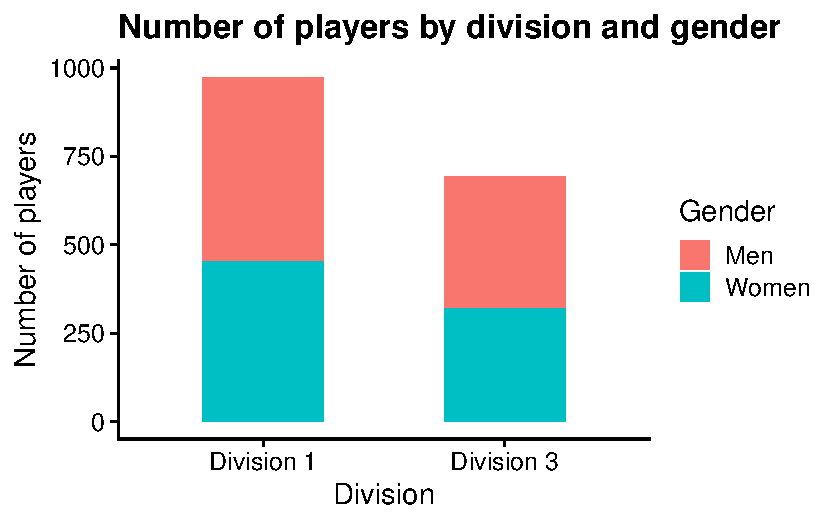
\includegraphics[keepaspectratio]{Julia_eda_files/figure-pdf/unnamed-chunk-1-1.pdf}}

\begin{Shaded}
\begin{Highlighting}[]
\NormalTok{df }\SpecialCharTok{\%\textgreater{}\%} \FunctionTok{ggplot}\NormalTok{(}\FunctionTok{aes}\NormalTok{(}\AttributeTok{x =}\NormalTok{ pts\_per\_game, }\AttributeTok{y =}\NormalTok{ plus\_minus, }\AttributeTok{color =}\NormalTok{ division)) }\SpecialCharTok{+} 
   \FunctionTok{geom\_point}\NormalTok{() }\SpecialCharTok{+} \FunctionTok{geom\_smooth}\NormalTok{(}\AttributeTok{method =} \StringTok{\textquotesingle{}lm\textquotesingle{}}\NormalTok{, }\AttributeTok{se =}\NormalTok{ F) }\SpecialCharTok{+} \FunctionTok{scale\_x\_log10}\NormalTok{() }\SpecialCharTok{+}
  \FunctionTok{labs}\NormalTok{(}\AttributeTok{x =} \StringTok{"Points per game"}\NormalTok{, }\AttributeTok{y =} \StringTok{"Plus/Minus"}\NormalTok{, }\AttributeTok{color =} \StringTok{"Division"}\NormalTok{) }\SpecialCharTok{+} 
  \FunctionTok{theme\_cowplot}\NormalTok{() }\SpecialCharTok{+}
  \FunctionTok{scale\_color\_viridis\_d}\NormalTok{()}
\end{Highlighting}
\end{Shaded}

\begin{verbatim}
Warning in scale_x_log10(): log-10 transformation introduced infinite values.
log-10 transformation introduced infinite values.
\end{verbatim}

\begin{verbatim}
`geom_smooth()` using formula = 'y ~ x'
\end{verbatim}

\begin{verbatim}
Warning: Removed 550 rows containing non-finite outside the scale range
(`stat_smooth()`).
\end{verbatim}

\pandocbounded{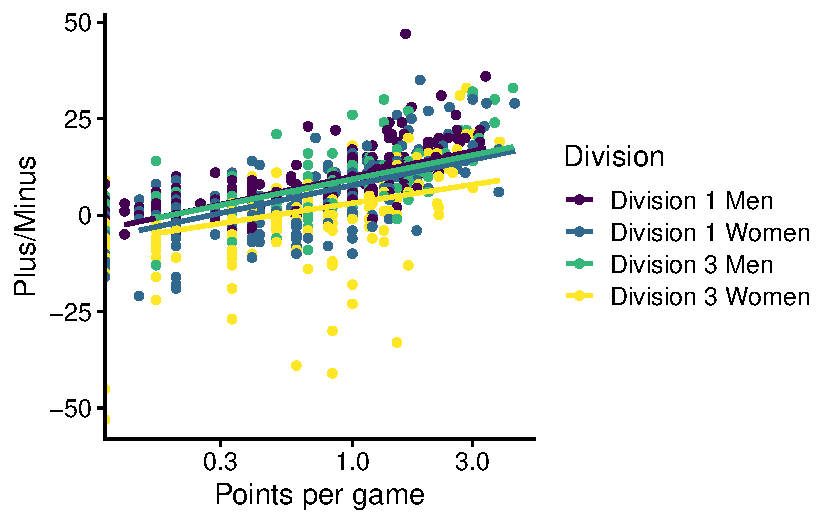
\includegraphics[keepaspectratio]{Julia_eda_files/figure-pdf/unnamed-chunk-2-1.pdf}}

\begin{Shaded}
\begin{Highlighting}[]
\NormalTok{df }\SpecialCharTok{\%\textgreater{}\%} \FunctionTok{ggplot}\NormalTok{(}\FunctionTok{aes}\NormalTok{(}\AttributeTok{x =}\NormalTok{ ds\_per\_game, }\AttributeTok{y =}\NormalTok{ plus\_minus, }\AttributeTok{color =}\NormalTok{ division)) }\SpecialCharTok{+} 
   \FunctionTok{geom\_point}\NormalTok{() }\SpecialCharTok{+} \FunctionTok{geom\_smooth}\NormalTok{(}\AttributeTok{method =} \StringTok{\textquotesingle{}lm\textquotesingle{}}\NormalTok{, }\AttributeTok{se =}\NormalTok{ F)}\SpecialCharTok{+}
  \FunctionTok{theme\_cowplot}\NormalTok{() }\SpecialCharTok{+} \FunctionTok{scale\_x\_log10}\NormalTok{() }\SpecialCharTok{+} 
  \FunctionTok{labs}\NormalTok{(}\AttributeTok{x =} \StringTok{"Ds per game"}\NormalTok{, }\AttributeTok{y =} \StringTok{"Plus/Minus"}\NormalTok{, }\AttributeTok{color =} \StringTok{"Division"}\NormalTok{) }\SpecialCharTok{+}
  \FunctionTok{scale\_color\_viridis\_d}\NormalTok{()}
\end{Highlighting}
\end{Shaded}

\begin{verbatim}
Warning in scale_x_log10(): log-10 transformation introduced infinite values.
log-10 transformation introduced infinite values.
\end{verbatim}

\begin{verbatim}
`geom_smooth()` using formula = 'y ~ x'
\end{verbatim}

\begin{verbatim}
Warning: Removed 638 rows containing non-finite outside the scale range
(`stat_smooth()`).
\end{verbatim}

\pandocbounded{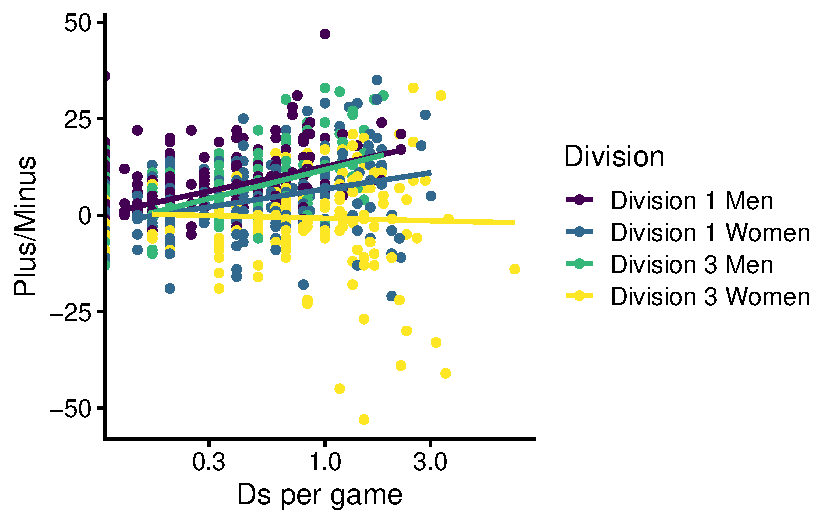
\includegraphics[keepaspectratio]{Julia_eda_files/figure-pdf/unnamed-chunk-2-2.pdf}}

\begin{Shaded}
\begin{Highlighting}[]
\NormalTok{df }\SpecialCharTok{\%\textgreater{}\%} \FunctionTok{ggplot}\NormalTok{(}\FunctionTok{aes}\NormalTok{(}\AttributeTok{x =}\NormalTok{ turns\_per\_game, }\AttributeTok{y =}\NormalTok{ plus\_minus, }\AttributeTok{color =}\NormalTok{ division)) }\SpecialCharTok{+} 
   \FunctionTok{geom\_point}\NormalTok{() }\SpecialCharTok{+} \FunctionTok{geom\_smooth}\NormalTok{(}\AttributeTok{method =} \StringTok{\textquotesingle{}lm\textquotesingle{}}\NormalTok{, }\AttributeTok{se =}\NormalTok{ F) }\SpecialCharTok{+} \FunctionTok{scale\_x\_log10}\NormalTok{() }\SpecialCharTok{+}
  \FunctionTok{labs}\NormalTok{(}\AttributeTok{x =} \StringTok{"Turns per game"}\NormalTok{, }\AttributeTok{y =} \StringTok{"Plus/Minus"}\NormalTok{, }\AttributeTok{color =} \StringTok{"Division"}\NormalTok{) }\SpecialCharTok{+} \FunctionTok{theme\_cowplot}\NormalTok{() }\SpecialCharTok{+}
  \FunctionTok{scale\_color\_viridis\_d}\NormalTok{()}
\end{Highlighting}
\end{Shaded}

\begin{verbatim}
Warning in scale_x_log10(): log-10 transformation introduced infinite values.
log-10 transformation introduced infinite values.
\end{verbatim}

\begin{verbatim}
`geom_smooth()` using formula = 'y ~ x'
\end{verbatim}

\begin{verbatim}
Warning: Removed 424 rows containing non-finite outside the scale range
(`stat_smooth()`).
\end{verbatim}

\pandocbounded{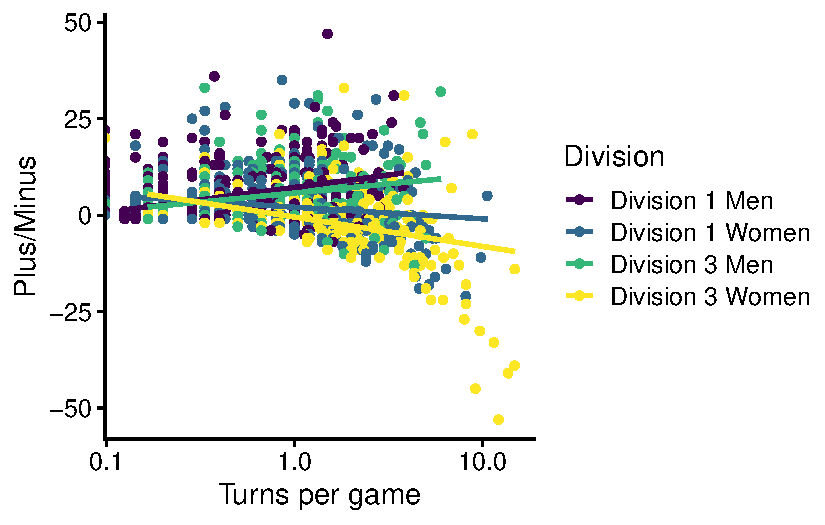
\includegraphics[keepaspectratio]{Julia_eda_files/figure-pdf/unnamed-chunk-2-3.pdf}}

\begin{Shaded}
\begin{Highlighting}[]
\NormalTok{df }\SpecialCharTok{\%\textgreater{}\%} \FunctionTok{ggplot}\NormalTok{(}\FunctionTok{aes}\NormalTok{(}\AttributeTok{x =}\NormalTok{ division, }\AttributeTok{y =}\NormalTok{ plus\_minus, }\AttributeTok{fill =}\NormalTok{ division)) }\SpecialCharTok{+} 
   \FunctionTok{geom\_boxplot}\NormalTok{() }\SpecialCharTok{+} \FunctionTok{scale\_y\_log10}\NormalTok{()}
\end{Highlighting}
\end{Shaded}

\begin{verbatim}
Warning in transformation$transform(x): NaNs produced
\end{verbatim}

\begin{verbatim}
Warning in scale_y_log10(): log-10 transformation introduced infinite values.
\end{verbatim}

\begin{verbatim}
Warning: Removed 729 rows containing non-finite outside the scale range
(`stat_boxplot()`).
\end{verbatim}

\pandocbounded{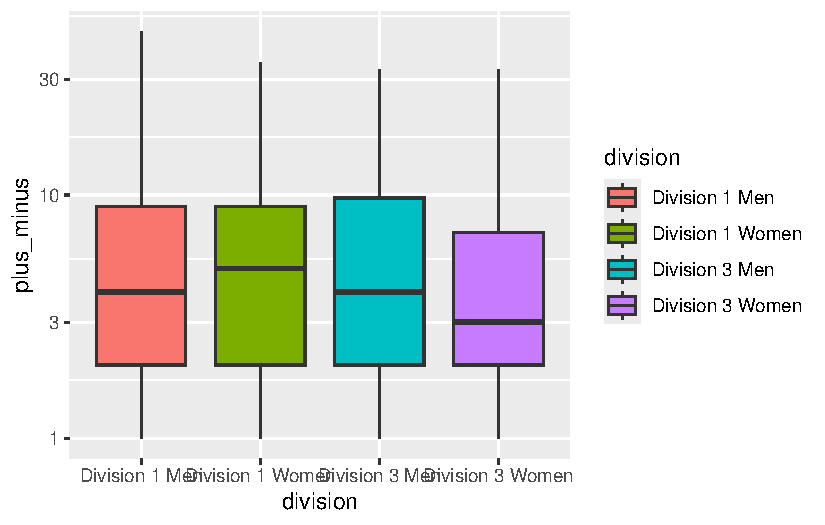
\includegraphics[keepaspectratio]{Julia_eda_files/figure-pdf/unnamed-chunk-3-1.pdf}}

\begin{Shaded}
\begin{Highlighting}[]
\NormalTok{df }\SpecialCharTok{\%\textgreater{}\%} \FunctionTok{ggplot}\NormalTok{(}\FunctionTok{aes}\NormalTok{(}\AttributeTok{x =}\NormalTok{ division, }\AttributeTok{y =}\NormalTok{ pts\_per\_game, }\AttributeTok{fill =}\NormalTok{ division)) }\SpecialCharTok{+} 
   \FunctionTok{geom\_boxplot}\NormalTok{() }\SpecialCharTok{+} \FunctionTok{scale\_y\_log10}\NormalTok{()}
\end{Highlighting}
\end{Shaded}

\begin{verbatim}
Warning in scale_y_log10(): log-10 transformation introduced infinite values.
\end{verbatim}

\begin{verbatim}
Warning: Removed 550 rows containing non-finite outside the scale range
(`stat_boxplot()`).
\end{verbatim}

\pandocbounded{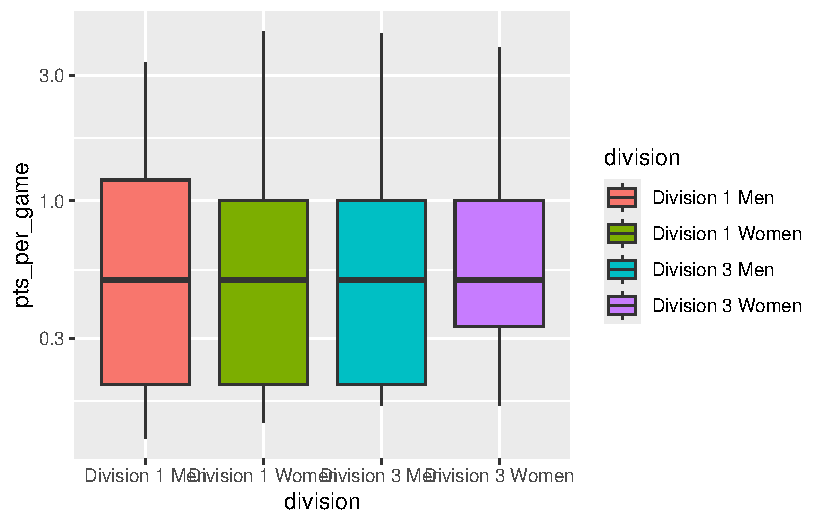
\includegraphics[keepaspectratio]{Julia_eda_files/figure-pdf/unnamed-chunk-3-2.pdf}}

\begin{Shaded}
\begin{Highlighting}[]
\FunctionTok{library}\NormalTok{(corrr)}
\end{Highlighting}
\end{Shaded}

\begin{verbatim}
Warning: package 'corrr' was built under R version 4.4.3
\end{verbatim}

\begin{Shaded}
\begin{Highlighting}[]
\FunctionTok{library}\NormalTok{(ggcorrplot)}
\end{Highlighting}
\end{Shaded}

\begin{verbatim}
Warning: package 'ggcorrplot' was built under R version 4.4.3
\end{verbatim}

\begin{Shaded}
\begin{Highlighting}[]
\FunctionTok{library}\NormalTok{(FactoMineR)}
\end{Highlighting}
\end{Shaded}

\begin{verbatim}
Warning: package 'FactoMineR' was built under R version 4.4.3
\end{verbatim}

\begin{Shaded}
\begin{Highlighting}[]
\FunctionTok{library}\NormalTok{(factoextra)}
\end{Highlighting}
\end{Shaded}

\begin{verbatim}
Warning: package 'factoextra' was built under R version 4.4.3
\end{verbatim}

\begin{verbatim}
Welcome! Want to learn more? See two factoextra-related books at https://goo.gl/ve3WBa
\end{verbatim}

\begin{Shaded}
\begin{Highlighting}[]
\FunctionTok{str}\NormalTok{(df)}
\end{Highlighting}
\end{Shaded}

\begin{verbatim}
'data.frame':   1665 obs. of  16 variables:
 $ player          : chr  "Jacques Nissen" "Cal Nightingale" "Faye Burdick" "Matthew Gregor" ...
 $ level           : Factor w/ 2 levels "Division 1","Division 3": 1 1 1 2 2 2 2 1 2 2 ...
 $ gender          : Factor w/ 2 levels "Men","Women": 1 1 2 1 2 1 2 1 1 1 ...
 $ division        : Factor w/ 4 levels "Division 1 Men",..: 1 1 2 3 4 3 4 1 3 3 ...
 $ team_name       : Factor w/ 70 levels "Alabama-Huntsville Nightmares",..: 5 5 18 21 13 20 13 5 70 53 ...
 $ Turns           : int  12 3 6 2 11 36 23 27 8 8 ...
 $ Ds              : int  8 0 12 6 15 7 20 6 11 4 ...
 $ Assists         : int  38 12 16 3 12 43 18 34 10 26 ...
 $ Points          : int  13 27 13 26 17 18 16 18 18 8 ...
 $ plus_minus      : int  47 36 35 33 33 32 31 31 31 30 ...
 $ team_games      : int  8 8 7 6 6 6 6 8 6 6 ...
 $ turns_per_game  : num  1.5 0.375 0.857 0.333 1.833 ...
 $ ds_per_game     : num  1 0 1.71 1 2.5 ...
 $ ast_per_game    : num  4.75 1.5 2.29 0.5 2 ...
 $ pts_per_game    : num  1.62 3.38 1.86 4.33 2.83 ...
 $ pls_mns_per_game: num  5.88 4.5 5 5.5 5.5 ...
\end{verbatim}

\begin{Shaded}
\begin{Highlighting}[]
\NormalTok{df1 }\OtherTok{\textless{}{-}}\NormalTok{ df }\SpecialCharTok{\%\textgreater{}\%} \FunctionTok{select}\NormalTok{(}\FunctionTok{c}\NormalTok{(}
\NormalTok{  turns\_per\_game, ds\_per\_game, pts\_per\_game, pls\_mns\_per\_game}
\NormalTok{))}

\NormalTok{pca }\OtherTok{\textless{}{-}}\NormalTok{ (}\FunctionTok{princomp}\NormalTok{(df1))}

\FunctionTok{fviz\_pca\_var}\NormalTok{(pca, }\AttributeTok{col.var =} \StringTok{"cos2"}\NormalTok{,}
            \AttributeTok{gradient.cols =} \FunctionTok{c}\NormalTok{(}\StringTok{"black"}\NormalTok{, }\StringTok{"orange"}\NormalTok{, }\StringTok{"green"}\NormalTok{),}
            \AttributeTok{repel =} \ConstantTok{TRUE}\NormalTok{)}
\end{Highlighting}
\end{Shaded}

\pandocbounded{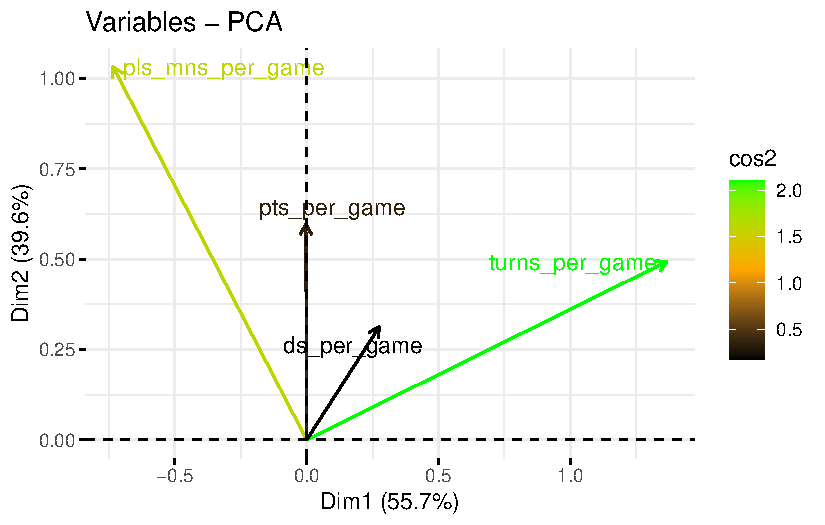
\includegraphics[keepaspectratio]{Julia_eda_files/figure-pdf/unnamed-chunk-4-1.pdf}}

\begin{Shaded}
\begin{Highlighting}[]
\FunctionTok{library}\NormalTok{(ggfortify)}
\end{Highlighting}
\end{Shaded}

\begin{verbatim}
Warning: package 'ggfortify' was built under R version 4.4.3
\end{verbatim}

\begin{Shaded}
\begin{Highlighting}[]
\NormalTok{pca\_df }\OtherTok{\textless{}{-}} \FunctionTok{prcomp}\NormalTok{(df1, }\AttributeTok{scale. =} \ConstantTok{TRUE}\NormalTok{)}
\FunctionTok{autoplot}\NormalTok{(pca\_df, }\AttributeTok{data =}\NormalTok{ df, }\AttributeTok{color =} \StringTok{"division"}\NormalTok{, }
         \AttributeTok{loadings =} \ConstantTok{TRUE}\NormalTok{, }\AttributeTok{loadings.label =} \ConstantTok{TRUE}\NormalTok{)}
\end{Highlighting}
\end{Shaded}

\pandocbounded{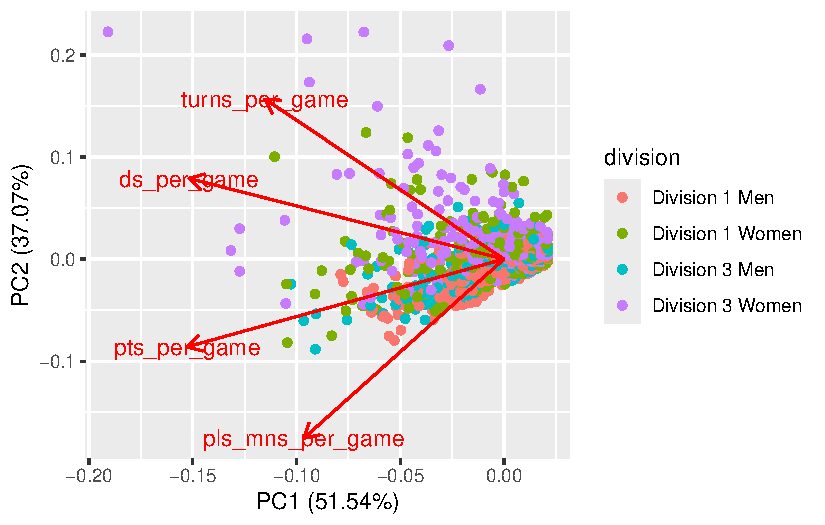
\includegraphics[keepaspectratio]{Julia_eda_files/figure-pdf/unnamed-chunk-4-2.pdf}}

\begin{Shaded}
\begin{Highlighting}[]
\FunctionTok{library}\NormalTok{(cluster)}
\FunctionTok{autoplot}\NormalTok{(}\FunctionTok{pam}\NormalTok{(df1[}\SpecialCharTok{{-}}\DecValTok{5}\NormalTok{], }\DecValTok{3}\NormalTok{), }\AttributeTok{frame =} \ConstantTok{TRUE}\NormalTok{)}
\end{Highlighting}
\end{Shaded}

\pandocbounded{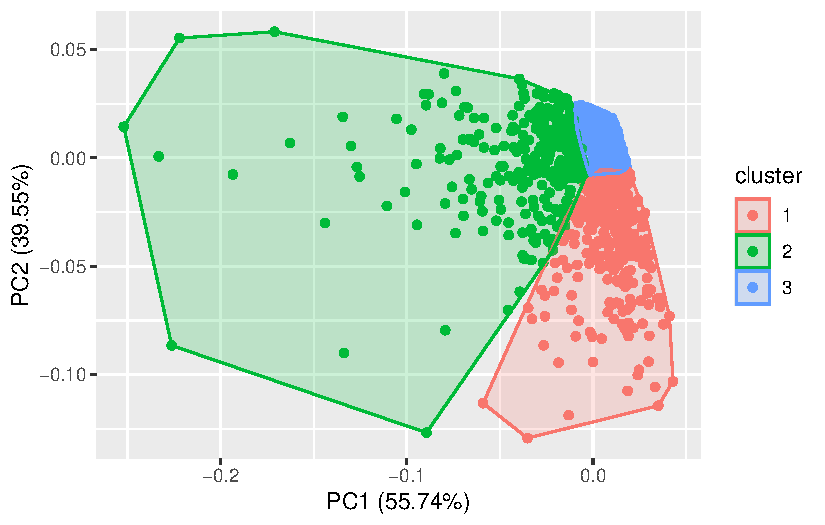
\includegraphics[keepaspectratio]{Julia_eda_files/figure-pdf/unnamed-chunk-4-3.pdf}}




\end{document}
